\documentclass[12pt]{article}                                                                                                                       
\usepackage{sbc-template}                                                 
\usepackage{graphicx,url}                                                 
\usepackage[utf8]{inputenc}                                               
\usepackage[brazil]{babel}                                                      
\usepackage{graphicx}

\title{Lista 1\\ Inteligência Artificial}
\author{Iyan Lucas Duarte Marques\inst{1}}

\address{Instituto de Ciências Exatas e Informática - Pontifícea Universidade Católica Minas Gerais (PUC-MG)}

\begin{document}

\maketitle

\section{Questão 01\\
Usando a base de restaurantee os parâmetros default do algoritmo J48, preencha os valores das seguintes métricas para esta base de dados a partir da árvore gerada pelo Weka
}
KDD é um processo conceitualizado por Fayyad com o objetivo de identificar padrões [validos] que possam ser utilizáveis na compreensão de dados.
\subsection{Processos}
\begin{itemize}
    \item \textbf{Análise da base}:
    Consiste na busca a compreensão da base de dados, qual a finalidade, atributos, campos, etc. 
    \item \textbf{Seleção e adição:}
    Consiste em selecionar um conjunto ou subconjunto de dados, dos quais os mesmos farão parte da análise pelo algorítmo.
    \item \textbf{Pre-processamento:}
    Consiste em validar a qualidade e a usabilidade do dado. 
    Sujeito à correção ou retirada dos dados inválidos do conjunto de dados usado.
    \item \textbf{Transformação:}
    Consiste em aplicar técnicas de transformação como: normalização, agregação, criação de novos atributos, redução e sintetização dos dados.
    Aqui os dados ficam disponíveis agrupados em um mesmo local para a aplicação dos modelos de análise.
    \item \textbf{Mineração de dados:}
    Consiste em construir modelos ou aplicar técnicas de mineração de dados. Essas técnicas têm por objetivo (1) verificar uma hipótese, (2) descobrir novos padrões de forma autônoma.
    Além disso, a descoberta pode ser dividida em: preditiva e descritiva.
    Esses modelos geralmente são aplicados e refeitos inúmeras vezes dependendo do objetivo do projeto.
    \item \textbf{Avaliação e interpretação:}
    Consiste em avaliar o desempenho do modelo, aplicando em cima de dados que não foram utilizados na fase de treinamento ou mineração.
    A validação pode ser feita de diversas formas, algumas delas são: utilizar medidas estatísticas, passar pela avaliação dos profissionais de negócio.
    \item \textbf{Visualização e integração:}
    Consiste na modelagem e \textit{plot} dos resultados obtidos nas etapas anteriores para visualização do cientista.
\end{itemize}

\section{Questão 02\\
Quais são os principais problemas de aprendizado de máquina existentes? Explique e
forneça exemplos.
}
\begin{itemize}
    \item \textbf{Classificação:} É um dos tipos de problemas mais utilizados que prevê ou descreve uma classe.
    O atributo de classificação é nominal.\\ 
    \textit{Exemplo:}\\

        \begin{tabular}{ l }
            \textbf{Chuva}\\
            \hline
          Sim \\ \hline
          Não \\ \hline
          Sim \\
          \hline
        \end{tabular}\\

    \item \textbf{Regressão:}
    Tal qual o problema de classificação porém seus atributos de classe são numéricos.\\
    \textit{Exemplo:}\\

    \begin{tabular}{ l }
        \textbf{Medalhas}\\
        \hline
      5 \\ \hline
      7 \\ \hline
      1 \\
      \hline
    \end{tabular}\\
    \item \textbf{Agrupamento (clusterização):}
    O problema busca agrupar as instâncias de acordo com os atributos de entrada.
    O problema não leva em consideração o atributo de classificação.\\
    \textit{Exemplo: Agrupar pessoas com interesses em comum ao planejar uma festa.}
    \item \textbf{Regras de associação:}
    O problema busca semelhanças e infere associações entre os elementos.\\
    \textit{Exemplo: Se uma pessoa escolheu x, também escolheu y.}

\end{itemize}


\section{Questão 03\\
Quais são os principais métodos de aprendizado existentes? Explique e forneça
exemplos.
}
\subsection{Supervisionado}
O indutor recebe conjunto de exemplos com uma entrada e um rótulo.
As técnicas utilizadas são:
\begin{itemize}
    \item Redes Neurais do tipo Multilayer Perceptron
    \item Máquinas de Vetores Suporte
    \item Árvores de Decisão
\end{itemize}

\subsection{Não Supervisionado}
O indutor recebe conjunto de exemplos somente com uma entrada e tenta encontrar agrupamentos.
\begin{itemize}
    \item Redes Neurais do tipo mapas auto-organizáveis
    \item Algoritmo k-médias
\end{itemize}

\subsection{Semi Supervisionado}
O indutor recebe conjunto de exemplos com uma entrada.
Os atributos podem ser ou não ser rotulados, cabe ao indutor decidir o melhor modelo.
\begin{itemize}
    \item SVM
\end{itemize}


\subsection{Reforço}
O indutor concentra-se na maximização das recompensas do resultado.
\begin{itemize}
    \item Redes Neurais
\end{itemize}

\subsection{\textit{Deep Learning}}
Rede neural com muitas camadas. Para cada reconhecendo
situações com ordem de complexidade maiores
\begin{itemize}
    \item Redes Neurais
\end{itemize}

\section{Questão 04\\
Considerando-se a base de dados sobre “Esperar ou não pelo restaurante” (verificar
base de dados disponibilizada no CANVAS), pede-se:
}
\subsection{Calcular o ganho de informação de cada atributo. Que atributo é a raiz da
árvore?
}
O atributo raiz da árvore é a coluna CLIENTE.
\subsection{Que atributo estará no segundo nível da árvore. Faça os cálculos e apresente a
árvore gerada.
}
O 2º atributo será a coluna SEX/SAB
\subsection{Quais as regras obtidas a partir desta árvore? Qual a cobertura de cada regra?
}


    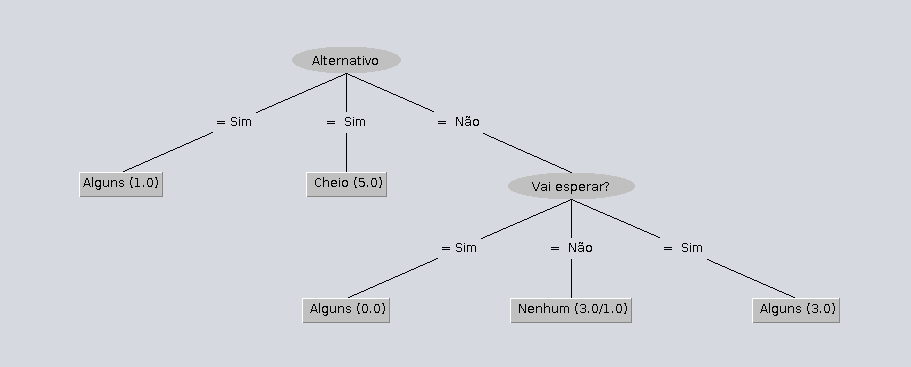
\includegraphics[width=\linewidth]{./ibagens/arvore.png}


\subsection{Rodar o algoritmo J48 do WEKA ou C4.5 de algum outro framework de
Machine Learning para verificar a árvore gerada.
}

\section{Questão 05}
\subsection{Utilizando-se a base de dados “Esperar ou não pelo restaurante”, altere os
parâmetros indicados na figura abaixo. Mande gerar a árvore novamente e veja o
que acontece. Explique.
PS: Para alterar algum parâmetro da função, clique sobre o nome da função, ao
lado da função “Choose”.
}
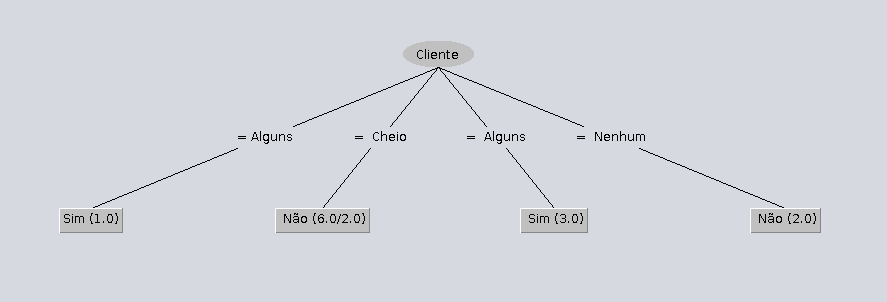
\includegraphics[width=\linewidth]{./ibagens/vai-esperar.png}

\subsection{Investigue o significado dos parâmetros ConfidenceFactor e NimNumObj
A opção More explica cada parâmetro.
}
\textit{\textbf{confidenceFactor} -- The confidence factor used for pruning (smaller values incur more pruning).}\\
\textit{\textbf{minNumObj} -- The minimum number of instances per leaf.}

\end{document}
